
\subsection{Variance equality tests}
\label{app:sec:variance}

In a more formal test, we investigate whether the variance of forecast errors is larger for foreign forecasters than the variance of local forecasters. To do this, we perform a simple variance equality test applied to the annual average of forecast errors across locations, defined as $\frac{1}{12}\sum_{m=1}^{12} Error_{ijt,t+h}^m$, for $h=0,1$. We use the annual average here to take into account a potential high correlation of the errors within a year, which could bias the test. We implement Levene’s variance equality test \citep{levene1960robust}. The null hypothesis, $H_0$, is that variances are equal $\sigma^2_{\text{FE}_{\text{Local}}} = \sigma^2_{\text{FE}_{\text{Foreign}}}$, versus the alternative hypothesis of unequal variances,  $H_A$, $\sigma^2_{\text{FE}_{\text{Local}}} \neq \sigma^2_{\text{FE}_{\text{Foreign}}}$.\footnote{Note that there are different ways for calculating the test statistic for equal variances, namely using the mean, median or trimmed mean. We observe very little differences across these methods which is why we report the results of the test statistics calculating with the mean.}


%the ratio of the standard deviation of the errors of local forecasters to that of foreign ones, and conduct a one-sided test with the null hypothesis, $H_0$, of equal variance, i.e. $\frac{\sigma_{\text{FE}_{\text{Local}}}}{\sigma_{\text{FE}_{\text{Foreign}}}} = 1$ versus the alternative hypothesis, $H_A$, that the ratio is $<1$.

{\setstretch{1}
\begin{table}[H] \centering
\newcolumntype{C}{>{\centering\arraybackslash}X}

\caption{Test for differences in Variance of Forecast Error}
\label{tab:error_sdtest}
{\footnotesize
\begin{tabularx}{\linewidth}{llCCCCCC}

\toprule
&{(1)}&{(2)}&{(3)}&{(4)}&{(5)}&{(6)}&{(7)} \tabularnewline \midrule
{Variable}&{Sample}&{ $ N $ Local}&{ $ N $ Foreign}&{ $ \sigma_\text{Local} $}&{ $\sigma_\text{Foreign} $}&{F-test}&{p-value} \tabularnewline
\midrule \addlinespace[0pt]
\midrule $ \text{CPI}_{t} $ &All sample&11,908&4,519&0.79&0.94&82.77&$< 0.001$ \tabularnewline
&Advanced Economies&5,655&1,278&0.42&0.49&29.39&$< 0.001$ \tabularnewline
&Emerging Economies&6,253&3,241&1.02&1.07&2.78&0.095 \tabularnewline
&Multinatonal firms&8,435&2,320&0.77&0.95&77.45&$< 0.001$ \tabularnewline
&National firms&3,473&2,199&0.86&0.93&12.74&$< 0.001$ \tabularnewline
&Financial Sector&8,005&1,274&0.78&1.04&69.99&$< 0.001$ \tabularnewline
&Non-Fincial Sector&1,828&2,158&0.74&0.83&19.10&$< 0.001$ \tabularnewline
$ \text{GDP}_{t} $ &All sample&12,390&4,701&1.15&1.44&131.49&$< 0.001$ \tabularnewline
&Advanced Economies&5,762&1,274&0.69&0.87&53.80&$< 0.001$ \tabularnewline
&Emerging Economies&6,628&3,427&1.44&1.60&15.36&$< 0.001$ \tabularnewline
&Multinatonal firms&8,690&2,424&1.11&1.51&148.38&$< 0.001$ \tabularnewline
&National firms&3,700&2,277&1.25&1.36&8.83&0.003 \tabularnewline
&Financial Sector&8,269&1,348&1.14&1.60&117.08&$< 0.001$ \tabularnewline
&Non-Fincial Sector&1,858&2,217&0.99&1.32&58.50&$< 0.001$ \tabularnewline
$ \text{CPI}_{t+1} $ &All sample&11,231&4,140&1.76&2.09&112.73&$< 0.001$ \tabularnewline
&Advanced Economies&5,382&1,171&0.91&1.04&22.85&$< 0.001$ \tabularnewline
&Emerging Economies&5,849&2,969&2.27&2.38&6.49&0.011 \tabularnewline
&Multinatonal firms&7,971&2,151&1.79&2.07&57.65&$< 0.001$ \tabularnewline
&National firms&3,260&1,989&1.68&2.10&60.22&$< 0.001$ \tabularnewline
&Financial Sector&7,582&1,192&1.81&2.17&44.28&$< 0.001$ \tabularnewline
&Non-Fincial Sector&1,711&1,964&1.66&2.00&45.50&$< 0.001$ \tabularnewline
$ \text{GDP}_{t+1} $ &All sample&11,707&4,341&2.45&3.10&109.10&$< 0.001$ \tabularnewline
&Advanced Economies&5,472&1,168&1.60&1.86&18.66&$< 0.001$ \tabularnewline
&Emerging Economies&6,235&3,173&3.00&3.45&15.99&$< 0.001$ \tabularnewline
&Multinatonal firms&8,206&2,275&2.36&3.24&123.84&$< 0.001$ \tabularnewline
&National firms&3,501&2,066&2.64&2.94&5.81&0.016 \tabularnewline
&Financial Sector&7,831&1,281&2.43&3.41&99.87&$< 0.001$ \tabularnewline
&Non-Fincial Sector&1,737&2,023&1.95&2.82&53.02&$< 0.001$ \tabularnewline
\bottomrule \addlinespace[\belowrulesep]

\end{tabularx}
\begin{flushleft}
\footnotesize \begin{minipage}{1\textwidth} \vspace{-10pt} \begin{tabnote} \textit{Notes:} The table shows Levene's variance equality test applied to the forecast errors of local and foreign forecasters. The Null hypothesis posits that the variance of the forecast errors made by local forecasters is equal to the  variance of the forecast errors made by foreign forecasters. The alternative hypothesis is that the variances are not equal. In the rows we report the test statistics for different subsamples. \end{tabnote} \end{minipage}  
\end{flushleft}
}
\end{table}

}

Table \ref{tab:error_sdtest} reports the results. In column (1), we define different sub-samples. We split the sample into advanced and emerging countries, multinational and national forecasters, financial and non-financial forecasters. Column (2) and (3) show the number of observations for local and foreign forecasters, respectively. Column (4) and (5) show the standard deviation of the forecast error conditional on the location. Column (6) reports the F-statistics and column (7) the corresponding p-value.


\newpage
\begin{figure}[h]
	
		\begin{subfigure}[b]{0.48\textwidth}
		\centering
		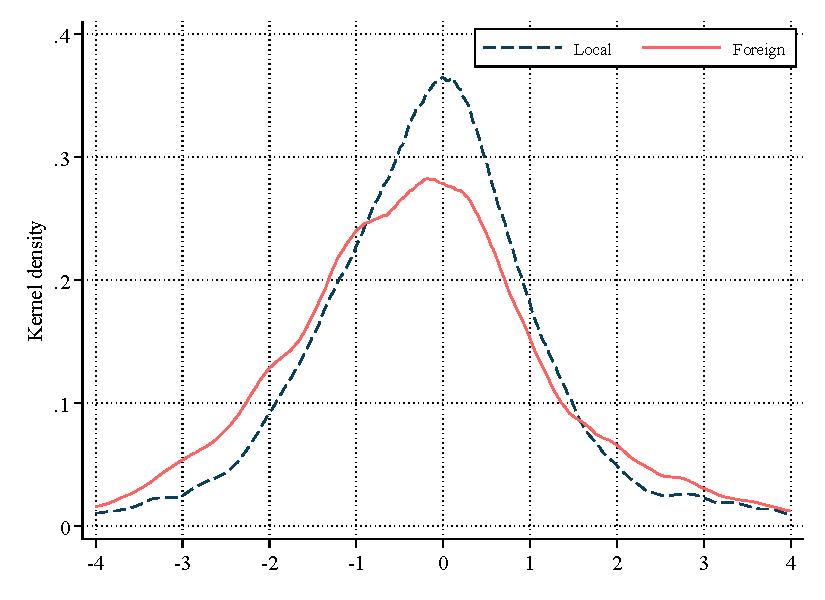
\includegraphics[width=1\linewidth]{Figures/cpi_future_FE_density}
		\caption{$Error_{ijt,t}^m$: $\text{CPI}_{t+1}$ }
		\label{fig:error_density_cpi_f}
	\end{subfigure}
	\hfill
	\begin{subfigure}[b]{0.48\textwidth}
		\centering
		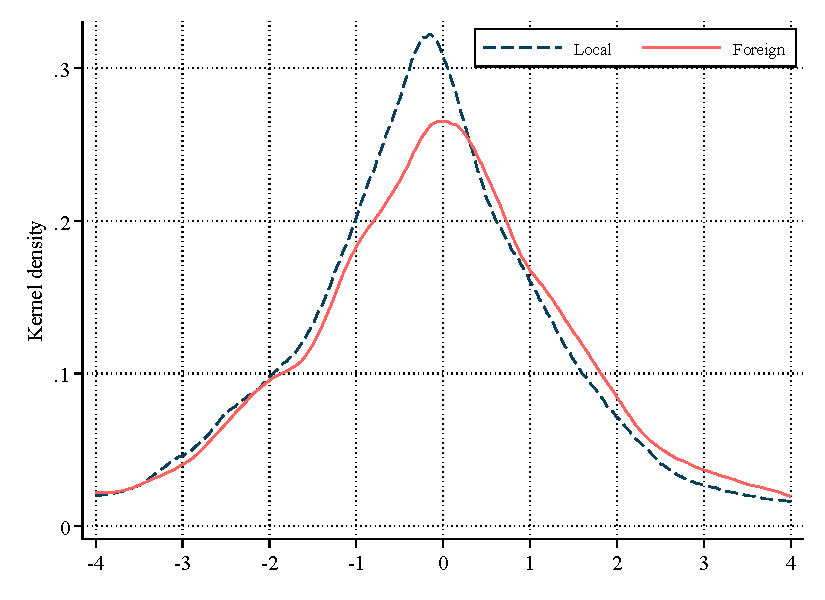
\includegraphics[width=1\linewidth]{Figures/gdp_future_FE_density}
		\caption{$Error_{ijt,t}^m$. $\text{GDP}_{t+1}$ }
		\label{fig:error_density_gdp_f}
	\end{subfigure}
	
	\begin{subfigure}[b]{0.48\textwidth}
		\centering
		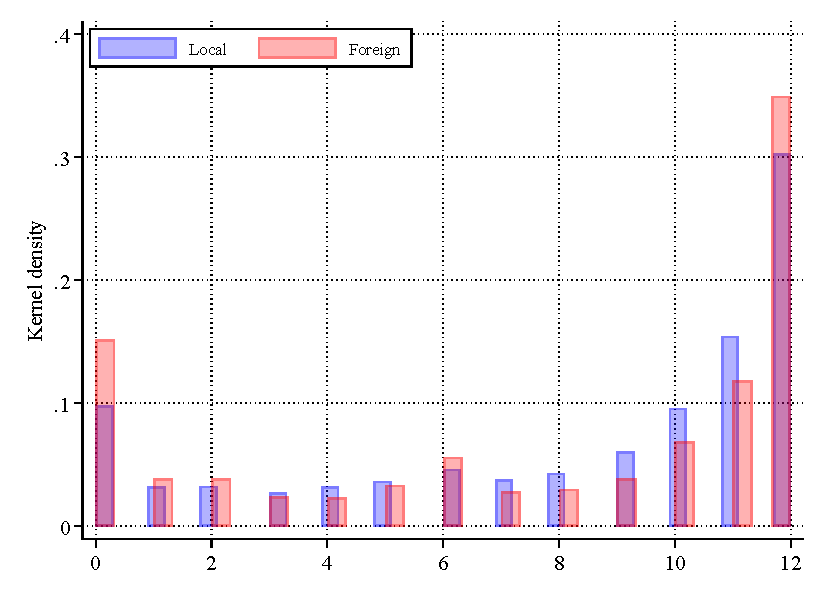
\includegraphics[width=1\linewidth]{Figures/cpi_future_N_density}
		\caption{$N_{ijt}$: $\text{CPI}_{t+1}$ }
		\label{fig:cpi_future_N_density}
	\end{subfigure}
	\hfill
	\begin{subfigure}[b]{0.48\textwidth}
		\centering
		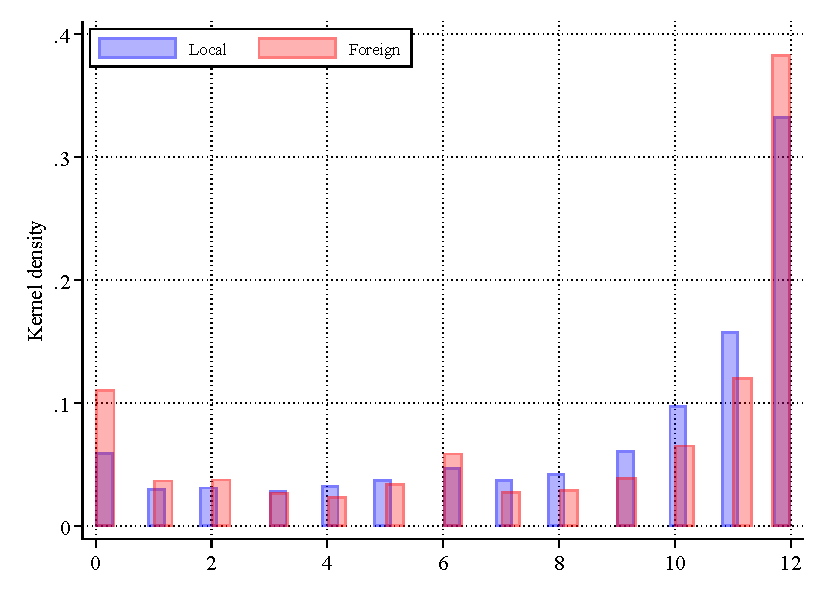
\includegraphics[width=1\linewidth]{Figures/gdp_future_N_density}
		\caption{$N_{ijt}$: $\text{GDP}_{t+1}$}
		\label{fig:gdp_future_N_density}
	\end{subfigure}
	
	\caption{Distribution of errors and distribution of the number of yearly updates}
	\label{fig:error_update_future}
	\begin{fignote}
		\textit{Notes:} Panels (a) and (b) display the density of the forecast error $Error_{ijt,t}^m$ conditional on the location of the forecaster. Panels (c) and (d) display the histograms of the number of updates $N_{ijt}$ by location. The population corresponds to all the country-forecaster-year units. We consider that any published forecast is an update.
	\end{fignote}
\end{figure}

{\setstretch{1}
\begin{table}[H] \centering
\newcolumntype{C}{>{\centering\arraybackslash}X}

\caption{Absolute Forecast Errors and the Location of the Forecaster - Alternative fixed effects}
\label{tab:tab_errors_rob}
{\footnotesize
\begin{tabularx}{\linewidth}{l l C C C C C}

\toprule
&&\multicolumn{5}{c}{$\ln(|Error_{ijt,t}^m|)$} \tabularnewline \cline{3-7} &\multicolumn{5}{c}{}& \multicolumn{1}{c}{Baseline}  \tabularnewline \cline{7-7} \tabularnewline &&{(1)}&{(2)}&{(3)}&{(4)}&{(5)} \tabularnewline
{Variable}&{Coefficient}&{}&{}&{}&{}&{} \tabularnewline
\midrule \addlinespace[0pt]
\midrule $ \text{CPI}_{t} $ &Foreign&0.26***&0.09***&0.10***&0.10***&0.09*** \tabularnewline
&&(0.08)&(0.03)&(0.03)&(0.02)&(0.02) \tabularnewline
&N&153,089&153,089&153,066&152,886&99,228 \tabularnewline
&$ R^2 $&0.01&0.11&0.14&0.55&0.62 \tabularnewline
$ \text{GDP}_{t} $ &Foreign&0.27***&0.02&0.11***&0.06**&0.06** \tabularnewline
&&(0.08)&(0.03)&(0.03)&(0.02)&(0.02) \tabularnewline
&N&160,971&160,971&160,947&160,765&103,866 \tabularnewline
&$ R^2 $&0.01&0.13&0.15&0.60&0.66 \tabularnewline
&Country FE&&\checkmark&\checkmark&& \tabularnewline
&Forecaster FE&&&\checkmark&\checkmark& \tabularnewline
&Country $ \times $ Date FE&&&&\checkmark&\checkmark \tabularnewline
&Forecaster $ \times $ Date FE &&&&&\checkmark \tabularnewline
\bottomrule \addlinespace[\belowrulesep]

\end{tabularx}
\begin{flushleft}
\footnotesize \begin{minipage}{1\linewidth} \vspace{-10pt} \begin{tabnote} \textit{Notes:} Columns (1) to (5) show the regression of the log absolute forecast error on the location of the forecaster with different fixed-effect specifications. Standard errors are clustered at the country, forecaster and date level. \end{tabnote} \end{minipage}  
\end{flushleft}
}
\end{table}
 
}

{\setstretch{1}
\begin{table}[H] \centering
\newcolumntype{C}{>{\centering\arraybackslash}X}

\caption{Forecast Errors, Updating, and the Location of the Forecaster - Future year}
\label{tab:updating_errors_app}
{\footnotesize
\begin{tabularx}{\linewidth}{l l C m{0.01\textwidth} C C C m{0.01\textwidth} C C C}

\toprule
{}&{}&{$\ln(\sigma^m_{\text{FE},i,j})$}&&\multicolumn{3}{c}{$\ln(|Error_{ijt+1,t}^m|)$}&&\multicolumn{3}{c}{$\ln(N_{ijt})$} \tabularnewline \cline{3-3} \cline{5-7} \cline{9-11} \tabularnewline &&{(1)}&&{(2)}&{(3)}&{(4)}&&{(5)}&{(6)}&{(7)} \tabularnewline
{Variable}&{Coefficient}&{}&{}&{}&{}&{}&{}&{}&{Distinct updates}&{} \tabularnewline
\midrule \addlinespace[0pt]
\midrule $\text{CPI}_{t+1}$&Foreign&0.07*&&0.07***&0.14**&0.06**&&--0.11***&--0.12***&0.07* \tabularnewline
&&(0.04)&&(0.02)&(0.06)&(0.03)&&(0.04)&(0.04)&(0.04) \tabularnewline
&&&&&&&&&&0.01 \tabularnewline
&&&&&&&&&&(0.03) \tabularnewline
&N&6,134&&90,693&13,208&72,978&&10,082&10,082&72,978 \tabularnewline
&$ R^2 $&0.86&&0.67&0.79&0.67&&0.53&0.51&0.67 \tabularnewline
$\text{GDP}_{t+1}$&Foreign&0.06**&&0.01&0.09&--0.00&&--0.10**&--0.10***&0.06 \tabularnewline
&&(0.03)&&(0.02)&(0.06)&(0.02)&&(0.04)&(0.03)&(0.05) \tabularnewline
&&&&&&&&&&0.07 \tabularnewline
&&&&&&&&&&(0.05) \tabularnewline
&N&6,565&&95,508&13,591&77,328&&10,464&10,464&77,328 \tabularnewline
&$ R^2 $&0.86&&0.72&0.79&0.73&&0.53&0.52&0.73 \tabularnewline
&Country, For., Month FE&\checkmark&&&&&&&& \tabularnewline
&Country $ \times $ Year FE&&&&&&&\checkmark&\checkmark& \tabularnewline
&Forecaster $ \times $ Year FE &&&&&&&\checkmark&\checkmark& \tabularnewline
&Country $ \times $ Date FE&&&\checkmark&\checkmark&\checkmark&&&&\checkmark \tabularnewline
&Forecaster $ \times $ Date FE &&&\checkmark&\checkmark&\checkmark&&&&\checkmark \tabularnewline
\bottomrule \addlinespace[\belowrulesep]

\end{tabularx}
\begin{flushleft}
\footnotesize \begin{minipage}{1\linewidth} \vspace{-10pt} \begin{tabnote} \textit{Notes:} Column (1) shows the regression of the log standard deviation of the errors on the location of the forecaster. Columns (2) to (4) show the regression of the log absolute forecast error on the location of the forecaster. Columns (5) and (7) show the results of regression of the number of forecast updates within a year on the location of the forecaster. Subsample 1 is restricted to the forecasts that are distinct from their last release. Subsample 2 is restricted to the forecasters that produce both local and foreign forecasts. Standard errors are clustered at the country and forecaster level in columns (1) and (5) to (7), and at the country, forecaster and date level in columns (2) to (4). \end{tabnote} \end{minipage}  
\end{flushleft}
}
\end{table}
 
}
